\documentclass[main.tex]{subfiles}
\begin{document}

% Full title as you would like it to appear on the page
\chapter{Long paper 1 chapter title}
% Short title that appears in the header of pages within the chapter
\chaptermark{Short chapter title}

\section{Abstract}
Concise introduction, motivation, results, and conclusions.

\section{Introduction}
Examples of citations: we knew X from \cite{Croote201616022} and Y from \cite{Croote20181306}.

\section{Results}
\subsection{Result 1}
Here is a reference to Figure \ref{fig:paper1_fig1}.
We found bacteria, roughly 5 \si{\mu}m in length, that live at 95\degree C for roughly 90\% of the year. More symbols: \$, \#, 10\textsuperscript{5}, $\alpha$, $\beta$, $\gamma$, $\kappa$, \textbf{bold}, \textit{italics}.
Quotation marks are "correctly oriented" thanks to the csquotes package.
Now an inline equation: $E = mc^2$. Now a reference to Equation \ref{eqn:paper1_eqn1}:
\begin{equation}\label{eqn:paper1_eqn1}
d_t = \frac{c - pn_t}{n_t}
\end{equation}

\begin{figure}[hbt!]
\centering
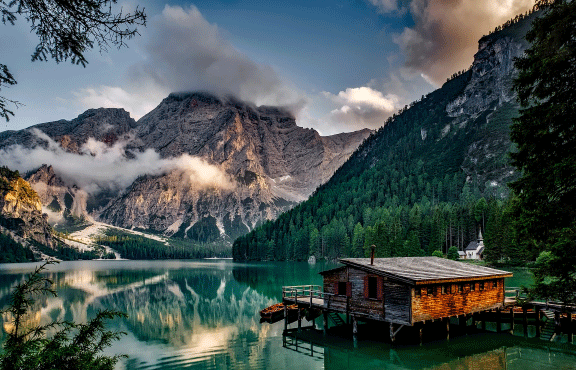
\includegraphics[width=14cm, keepaspectratio]{paper1/fig1.png}
\caption[Short figure caption for List of Figures]{Long figure caption text that explains everything.}
\label{fig:paper1_fig1}
\end{figure}

There will be more text here.

More text here.

More text here.

More text here.

More text here.

More text here.

\subsection{Result 2}
We discovered something else. Here is a reference to Table \ref{tab:paper1_tab1}.

\renewcommand{\arraystretch}{2}  % make spacing nicer
\begin{table}[hbt!]
\centering
\begin{tabularx}{\textwidth}{c|c|c|c}  % 4 columns center-justified
   \textbf{Col 1} & \textbf{Col 2} & \textbf{Col 3} & \textbf{Col 4} \\
   \hline  % horizontal line
   Text in Row 1a & Text in Row 1b & Text in Row 1c & Lots of text in Row 1d \\
                  & Row 1.5b & Row 1.5c & Row 1.5d \\
   \hline
   Row 2a & Row 2b & Row 2c & Row 2d \\
   \hline
   Row 3a & Row 3b & Row 3c & Row 3d \\
\end{tabularx}
\caption[Short table caption for List of Tables]{Long table caption explaining everything.}
\label{tab:paper1_tab1}
\end{table}

More text here.

More text here.

More text here.

More text here.

\begin{sloppypar}
FixAwkwardSpacingWithSloppypar FixAwkwardSpacingWithSloppypar FixAwkwardSpacingWithSloppypar FixAwkwardSpacingWithSloppypar FixAwkwardSpacingWithSloppypar.
\end{sloppypar}

More text here.

More text here.

\section{Conclusions}
The end of the paper.

% Uncomment to print the bibliography when compiling individual chapters
\iftoggle{biblatex}{
  \ifSubfilesClassLoaded{\printbibliography}{}
}{
  \ifSubfilesClassLoaded{\bibliography{../bib/mybib}}{}
}
\end{document}
